\section{Results}
\label{sec:results}

Every number in this section is computed by \texttt{tools/analyse.py} from the
runs' logs; the design log (28 and 29 October) records how each was first
read.

\subsection{Evaluation: model and plan}
\label{sec:evaluation}

\Cref{tab:evaluation} gives the evaluation: 20 drones and 2 leaders on the
two held-out maps.

\begin{table}[tbp]
  \centering
  \small
  \begin{tabular}{@{}lcccc@{}}
    \toprule
    & \multicolumn{2}{c}{\texttt{dead\_end} (83\,s)} & \multicolumn{2}{c}{\texttt{l\_turn} (112\,s)} \\
    \cmidrule(lr){2-3}\cmidrule(l){4-5}
    & plan off & plan on & plan off & plan on \\
    \midrule
    hybrid   & 0/10        & 2/10 (47\,s) & 10/10 (68\,s) & 10/10 (66\,s) \\
    Couzin   & 3/10 (73\,s) & 6/10 (57\,s) & 9/10 (75\,s)  & 9/10 (75\,s) \\
    Reynolds & 0/10        & 8/10 (56\,s) & 0/10          & 10/10 (69\,s) \\
    \bottomrule
  \end{tabular}
  \caption{Evaluation, 20 drones, 2 leaders: runs out of 10 seeds with 90\% of
    the drones in C within the limit, and the median time to 90\% of those
    runs.}
  \label{tab:evaluation}
\end{table}

\paragraph{The plan.} With the plan, Reynolds' flock reaches C in 8 of 10 runs
on \texttt{dead\_end} and in all 10 on \texttt{l\_turn}, from none on either
map without it (paired: 8 seeds to none, $p = 0.008$; 10 to none,
$p = 0.002$). This confirms H2: the trap at the corner is steering straight at
C, not Reynolds' rules, since the same rules get round it as soon as the
leaders follow a path. For the hybrid and Couzin the plan's effect is small
(2 seeds to none, and 4 to 1, $p \ge 0.37$): on \texttt{l\_turn} both already
succeed without it, because their flocks' own momentum carries the leaders
round the corner; on \texttt{dead\_end} the hybrid stays low either way. H1
holds for Reynolds and is not shown for the other two; its second part, no
effect where the way to C is clear, was not tested.

\paragraph{The models.} With the plan off, the hybrid and Couzin beat Reynolds
on \texttt{l\_turn} (10 and 9 seeds to none, $p \le 0.004$). With the plan on,
the order on \texttt{dead\_end} reverses: Reynolds 8, Couzin 6, the hybrid 2.
Hybrid against Reynolds is 6 seeds to none ($p = 0.03$). In the hybrid's 8
failures only 1 or 2 drones, its leaders, are in C at the limit:
\cref{sec:split} shows why. Couzin succeeds where the other two don't with
the plan off (3 runs), and loses its flock in a few runs with the plan on, as
expected from its tuning: its leaders, off the walls, can leave the flock
behind.

\paragraph{Spacing.} \Cref{fig:evaluation-closest} shows the closest two
drones came in each run. Reynolds keeps its drones apart, 0.42--0.51\,m in
median, never closer than 0.33\,m. The hybrid and Couzin crowd to touching
distance, 0.10\,m, in many runs, and Couzin is the only model that crashed (4
runs of 40; the plan-off runs were measured over 200\,s). So H3 holds for
reaching C, where tuned Couzin matches the hybrid, but not for spacing:
Couzin's drones are no further apart than the hybrid's. The plan widens the
hybrid's spacing on both maps (Wilcoxon, $p \le 0.004$): a flock that presses
into a wall is a compressed flock.

\begin{figure}[tbp]
  \centering
  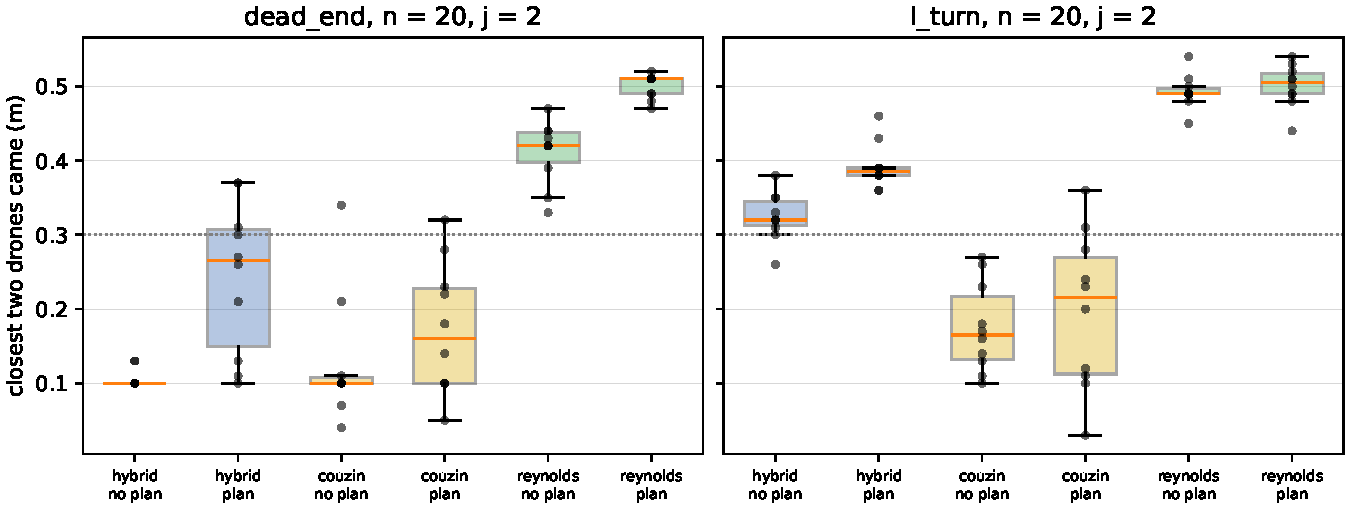
\includegraphics[width=\linewidth]{evaluation_closest}
  \caption{The closest two drones came in each run, on the held-out maps with
    20 drones and 2 leaders, 10 seeds. Dotted: the 0.3\,m stopping margin;
    0.10\,m is touching.}
  \label{fig:evaluation-closest}
\end{figure}

\subsection{Drones and leaders}
\label{sec:sweep}

\Cref{fig:sweep-success} shows the second experiment, on \texttt{dead\_end}
with the plan on, and \cref{tab:leaders} pools it over the three flock sizes.

\begin{figure}[tbp]
  \centering
  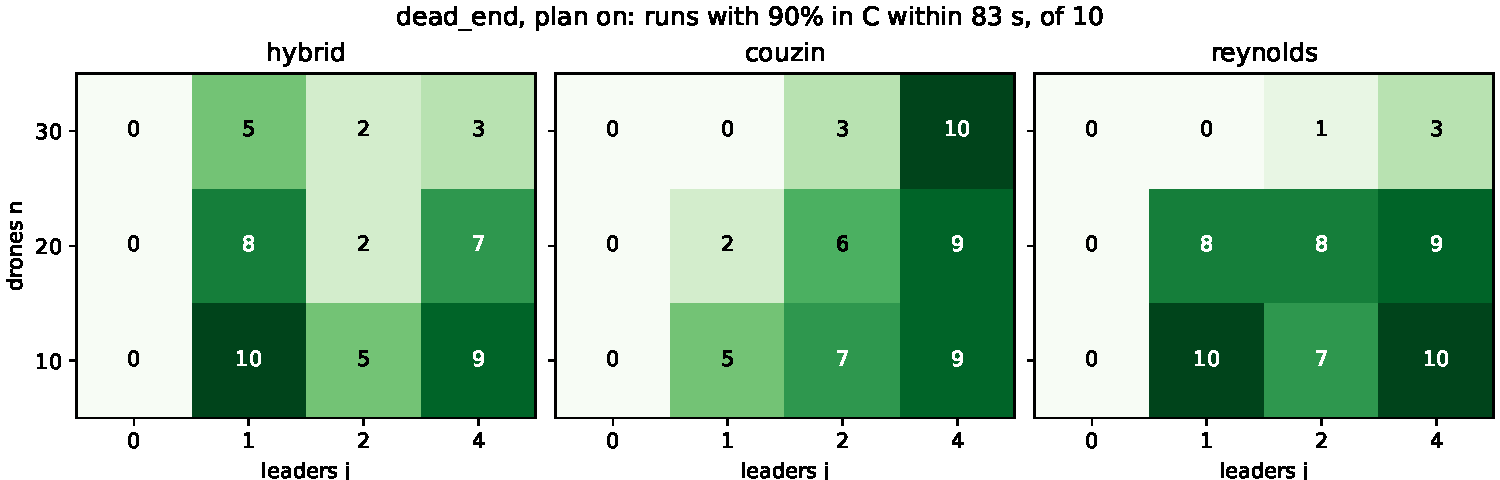
\includegraphics[width=\linewidth]{sweep_success}
  \caption{\texttt{dead\_end} with the plan: runs out of 10 seeds with 90\% of
    the drones in C within 83\,s, by flock size $n$ and leaders $j$.}
  \label{fig:sweep-success}
\end{figure}

\begin{table}[tbp]
  \centering
  \small
  \begin{tabular}{@{}lccccl@{}}
    \toprule
    & $j = 0$ & $j = 1$ & $j = 2$ & $j = 4$ & paired, $j = 1$ vs 4 \\
    \midrule
    hybrid   & 0/30 & 23/30 & 9/30  & 19/30 & 4 / 8 seeds, $p = 0.39$ \\
    Couzin   & 0/30 & 7/30  & 16/30 & 28/30 & 22 / 1 seeds, $p < 10^{-5}$ \\
    Reynolds & 0/30 & 18/30 & 16/30 & 22/30 & 5 / 1 seeds, $p = 0.22$ \\
    \bottomrule
  \end{tabular}
  \caption{\texttt{dead\_end} with the plan, pooled over $n = 10, 20, 30$:
    successful runs out of 30, and the paired test of 1 leader against 4
    (seeds won by $j = 4$ / by $j = 1$).}
  \label{tab:leaders}
\end{table}

\paragraph{No leaders, no arrival.} None of the 90 runs with $j = 0$ reached C
within the limit. Every success in the experiment is the leaders' doing: the
chance level the time limit was set to remove is zero.

\paragraph{More leaders.} Couzin's model behaves as \citet{couzin2005}
predict: its flock follows more reliably the more leaders it has, 7, 16 and
28 runs of 30 for 1, 2 and 4 leaders (from 1 to 2: 11 seeds to 2,
$p = 0.02$; from 2 to 4: 13 to 1, $p = 0.002$), and at $n = 30$ it is the
only model that still succeeds reliably, 10 of 10 with 4 leaders against 3 for
the other two. With one leader its flock packs to touching distance and does
not follow. Reynolds hardly depends on $j$ (18, 16, 22 of 30; every pair
$p \ge 0.07$). The hybrid does worse with 2 leaders than with 1: 23 of 30
against 9, 14 seeds to none ($p = 0.0001$), and recovers with 4. H4 holds for
Couzin's model only.

\paragraph{Larger flocks.} Every model succeeds less with more drones (over
$j > 0$: the hybrid 24, 17, 10 runs of 30 from $n = 10$ to 30; Couzin 21, 17,
13; Reynolds 27, 25, 4). With $j$ fixed, the fraction of leaders falls as $n$
grows, so this does not contradict Couzin's result that larger groups need a
\emph{smaller fraction}; it says that, here, they need more than a constant
number. Reynolds' collapse at $n = 30$ is the sharpest: from 25 of 30 to 4.

\paragraph{Cost.} \Cref{fig:sweep-cost} shows what success costs. Reynolds
arrives in about the same time as the others (median 51--54\,s against
47--60\,s) with its drones twice as far apart (median closest pair about
0.5\,m). Couzin with one leader sits at 0.10\,m; with more leaders its
spacing widens to the hybrid's. The hybrid with 4 leaders is the slowest
(median 60\,s).

\begin{figure}[tbp]
  \centering
  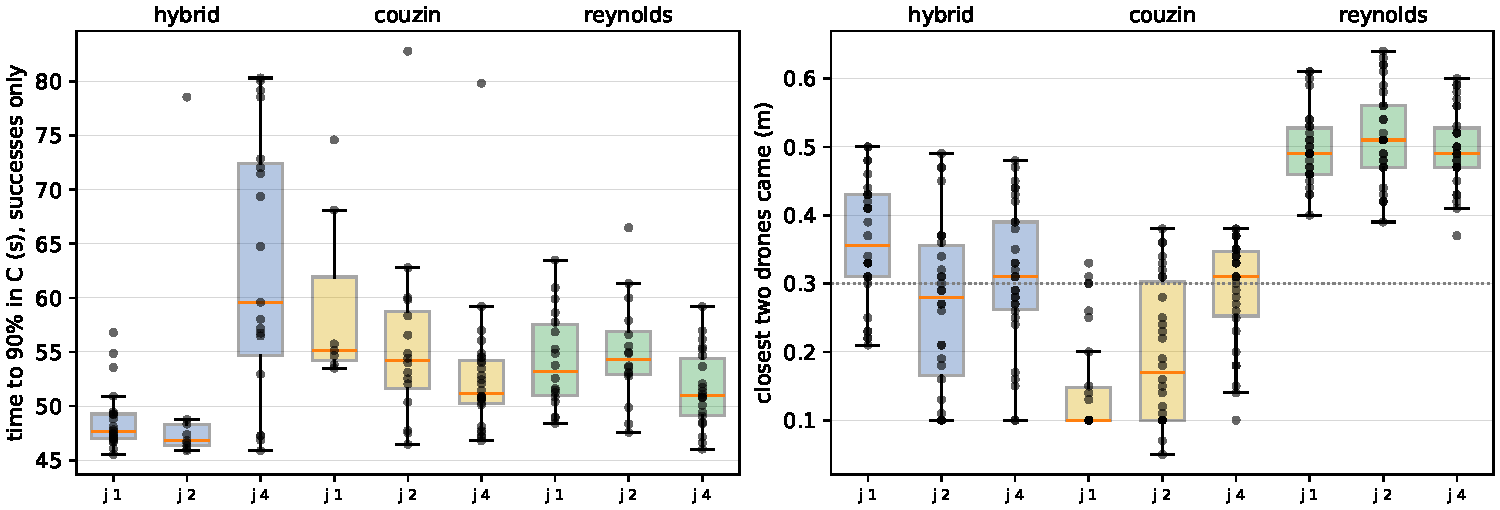
\includegraphics[width=\linewidth]{sweep_cost}
  \caption{\texttt{dead\_end} with the plan, pooled over flock sizes: the time
    to 90\% in C of the successful runs (left) and the closest two drones came
    in every run (right), per model and number of leaders.}
  \label{fig:sweep-cost}
\end{figure}

\subsection{Why two leaders lose the hybrid's flock}
\label{sec:split}

A failure of the hybrid with 2 leaders that Reynolds, on the same spawn,
turns into a success, replayed and drawn in \cref{fig:split}, shows the
mechanism.

\begin{enumerate}
  \item The two leaders start on either side of the cup's axis, and each
        plans round its own arm of the cup, one over the top, one under the
        bottom. Their paths part slowly, so at go time both still head
        roughly east.
  \item The hybrid's followers cruise along the mean heading of their
        neighbours, and they are at full speed within 2\,s of the start. The
        two leaders' pulls, up and down, cancel, so the followers fly straight
        on, overtake both leaders and fill the cup.
  \item At the bottom of the cup they turn back as one, carry the top leader
        with them (a leader mixes the goal with its neighbours' heading), and
        loop round the room. The bottom leader reaches C alone.
  \item Reynolds' followers have no cruise: they speed up only as their
        neighbours pull them (0.34\,m/s at 18\,s, against the hybrid's
        0.99). The leaders get ahead and apart before the flock commits, and
        the flock goes with one of them, over the top arm, into C.
\end{enumerate}

This is the averaging \citet{couzin2005} found in groups with two informed
subgroups: when their preferred directions differ only a little, the group
follows their mean, and only a wide enough difference makes it choose one.
Here the difference starts small, two paths that part slowly, and their mean
leads into the dead end.

\begin{figure}[tbp]
  \centering
  \begin{subfigure}{\linewidth}
    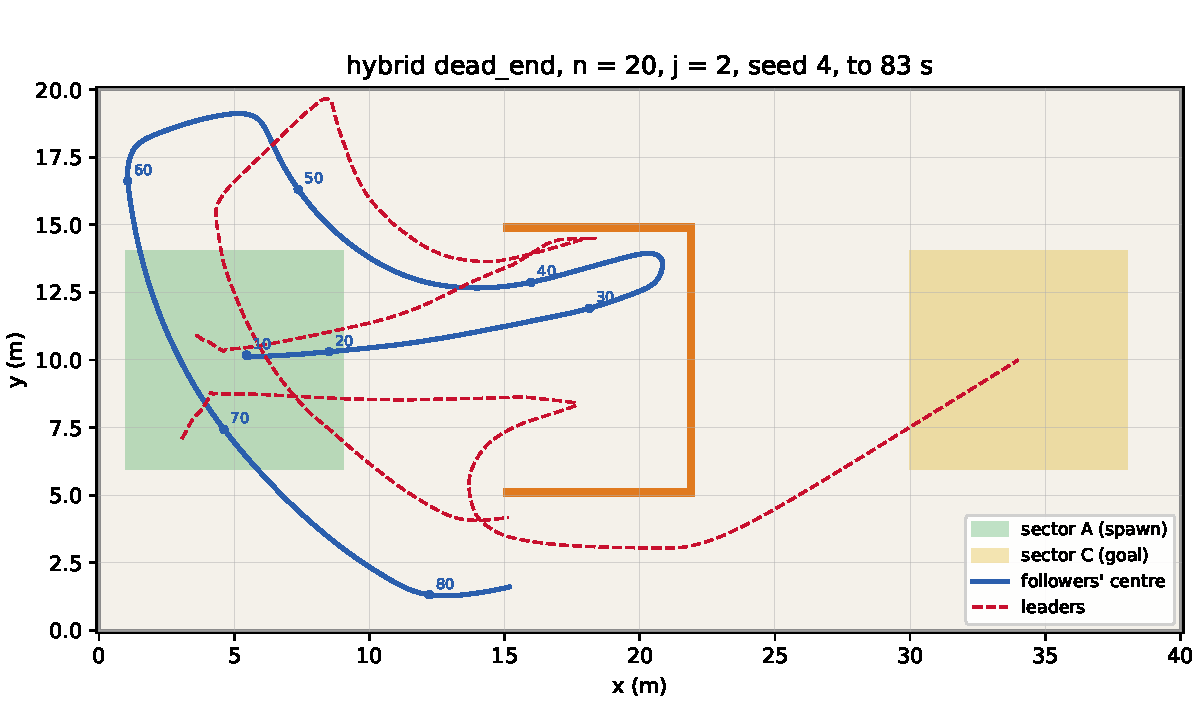
\includegraphics[width=\linewidth]{trajectory_dead_end_hybrid_plan_n20_j2_seed4}
    \caption{Hybrid: the followers fly between the two leaders into the cup,
      then loop round the room with the top leader.}
  \end{subfigure}
  \begin{subfigure}{\linewidth}
    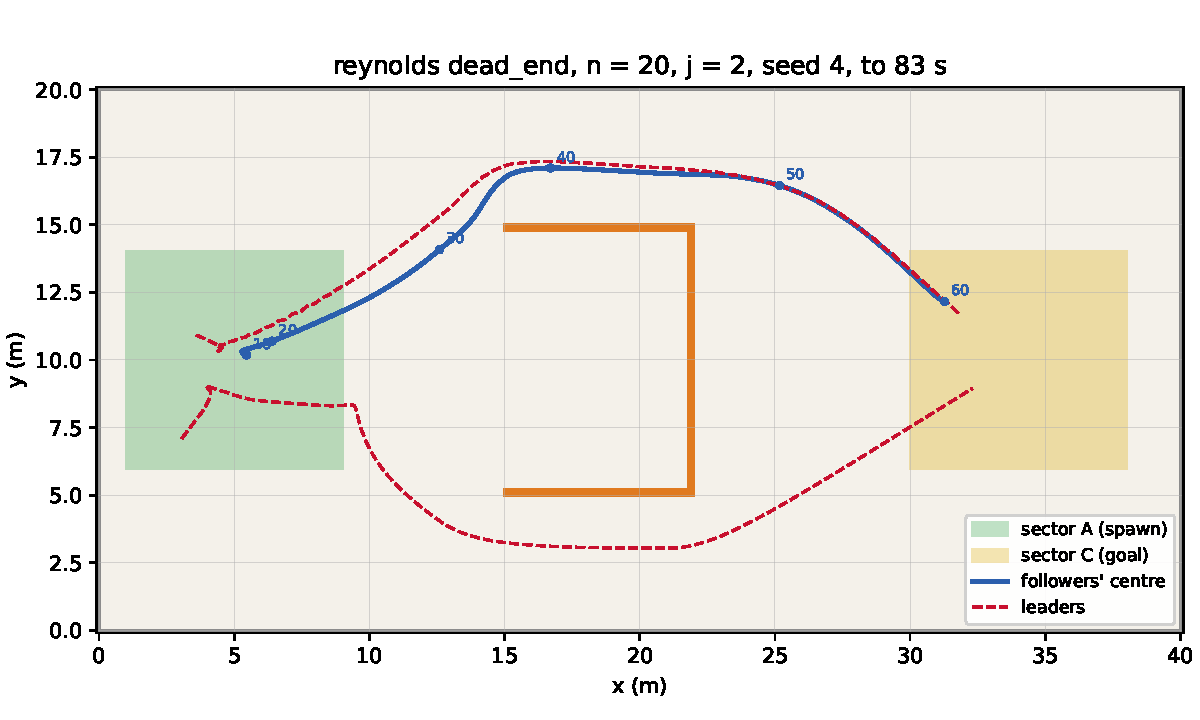
\includegraphics[width=\linewidth]{trajectory_dead_end_reynolds_plan_n20_j2_seed4}
    \caption{Reynolds: the followers go with the top leader into C.}
  \end{subfigure}
  \caption{The same spawn (seed 4, 20 drones, 2 leaders) with two models, to
    the 83\,s limit. Solid: the followers' centre, numbered every 10\,s;
    dashed: the leaders.}
  \label{fig:split}
\end{figure}

\paragraph{Over all runs.} A* is deterministic and a leader plans from within
a metre of where it spawned, so planning from each leader's spawn tells which
way it went. \Cref{tab:split} relates that to success for the runs with 2
leaders.

\begin{table}[tbp]
  \centering
  \small
  \begin{tabular}{@{}lccc@{}}
    \toprule
    & same way (10 runs) & opposite ways (20 runs) & Fisher's exact $p$ \\
    \midrule
    hybrid   & 7/10 & 2/20  & 0.002 \\
    Couzin   & 7/10 & 9/20  & 0.26 \\
    Reynolds & 5/10 & 11/20 & 1.0 \\
    \bottomrule
  \end{tabular}
  \caption{\texttt{dead\_end} with the plan, 2 leaders, $n = 10, 20, 30$:
    successful runs when both leaders plan round the same side of the cup and
    when they plan round opposite sides.}
  \label{tab:split}
\end{table}

Only the hybrid is broken by the split: with its leaders on one side it
succeeds as often as the others. Couzin's and Reynolds' flocks choose a
leader. With 4 leaders the hybrid recovers (19 of 30); an even 2--2 split
does not break it the same way (8 of 12 runs), which this analysis does not
explain.

\todo{Video: the hybrid and Reynolds on seed 4, side by side.}
